\subsection{Entity-Relationship Schema}

We decided to start our project starting from the database designed by the e-team group during the FTB course. We report in the following figures the design from we started. In particular in figure \ref{er_original} we reported the ER schema and in figure \ref{ls_original} the corresponding relational schema.

\begin{figure}[H]
\centering
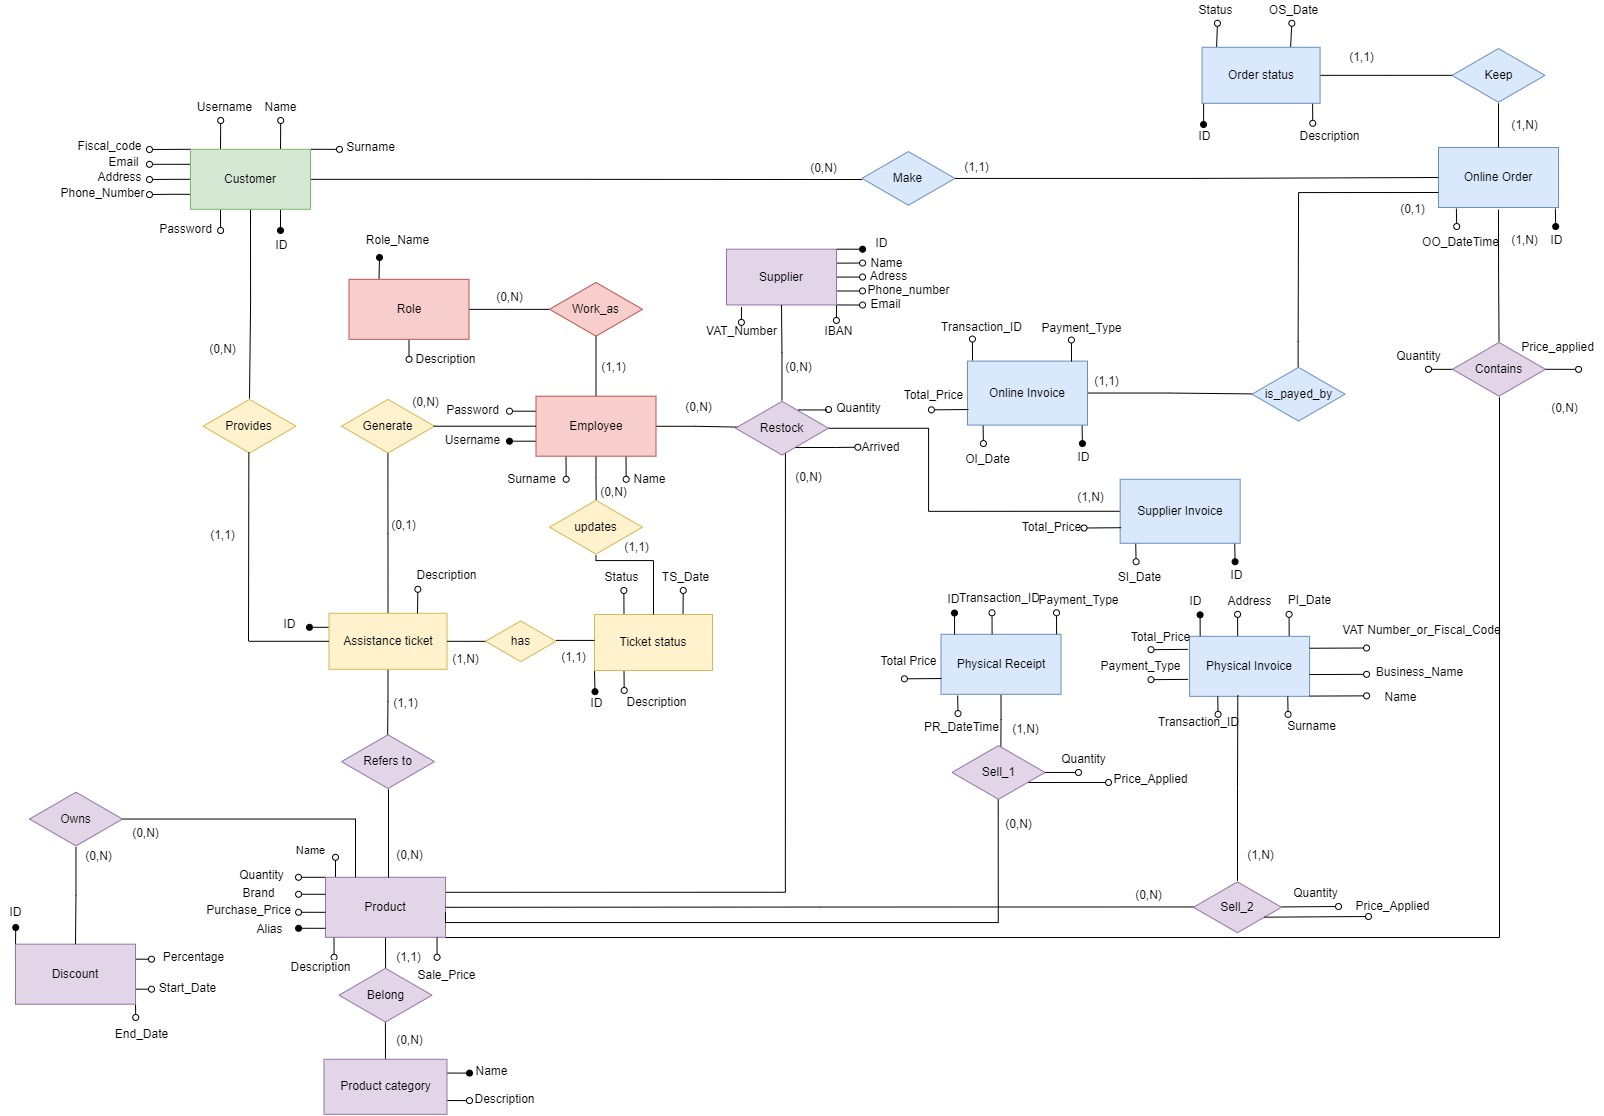
\includegraphics[width=17cm]{Schemas/ER_original.jpg}
\caption{ER schema designed by e-team}
\label{er_original}
\end{figure}

\begin{figure}[H]
\centering
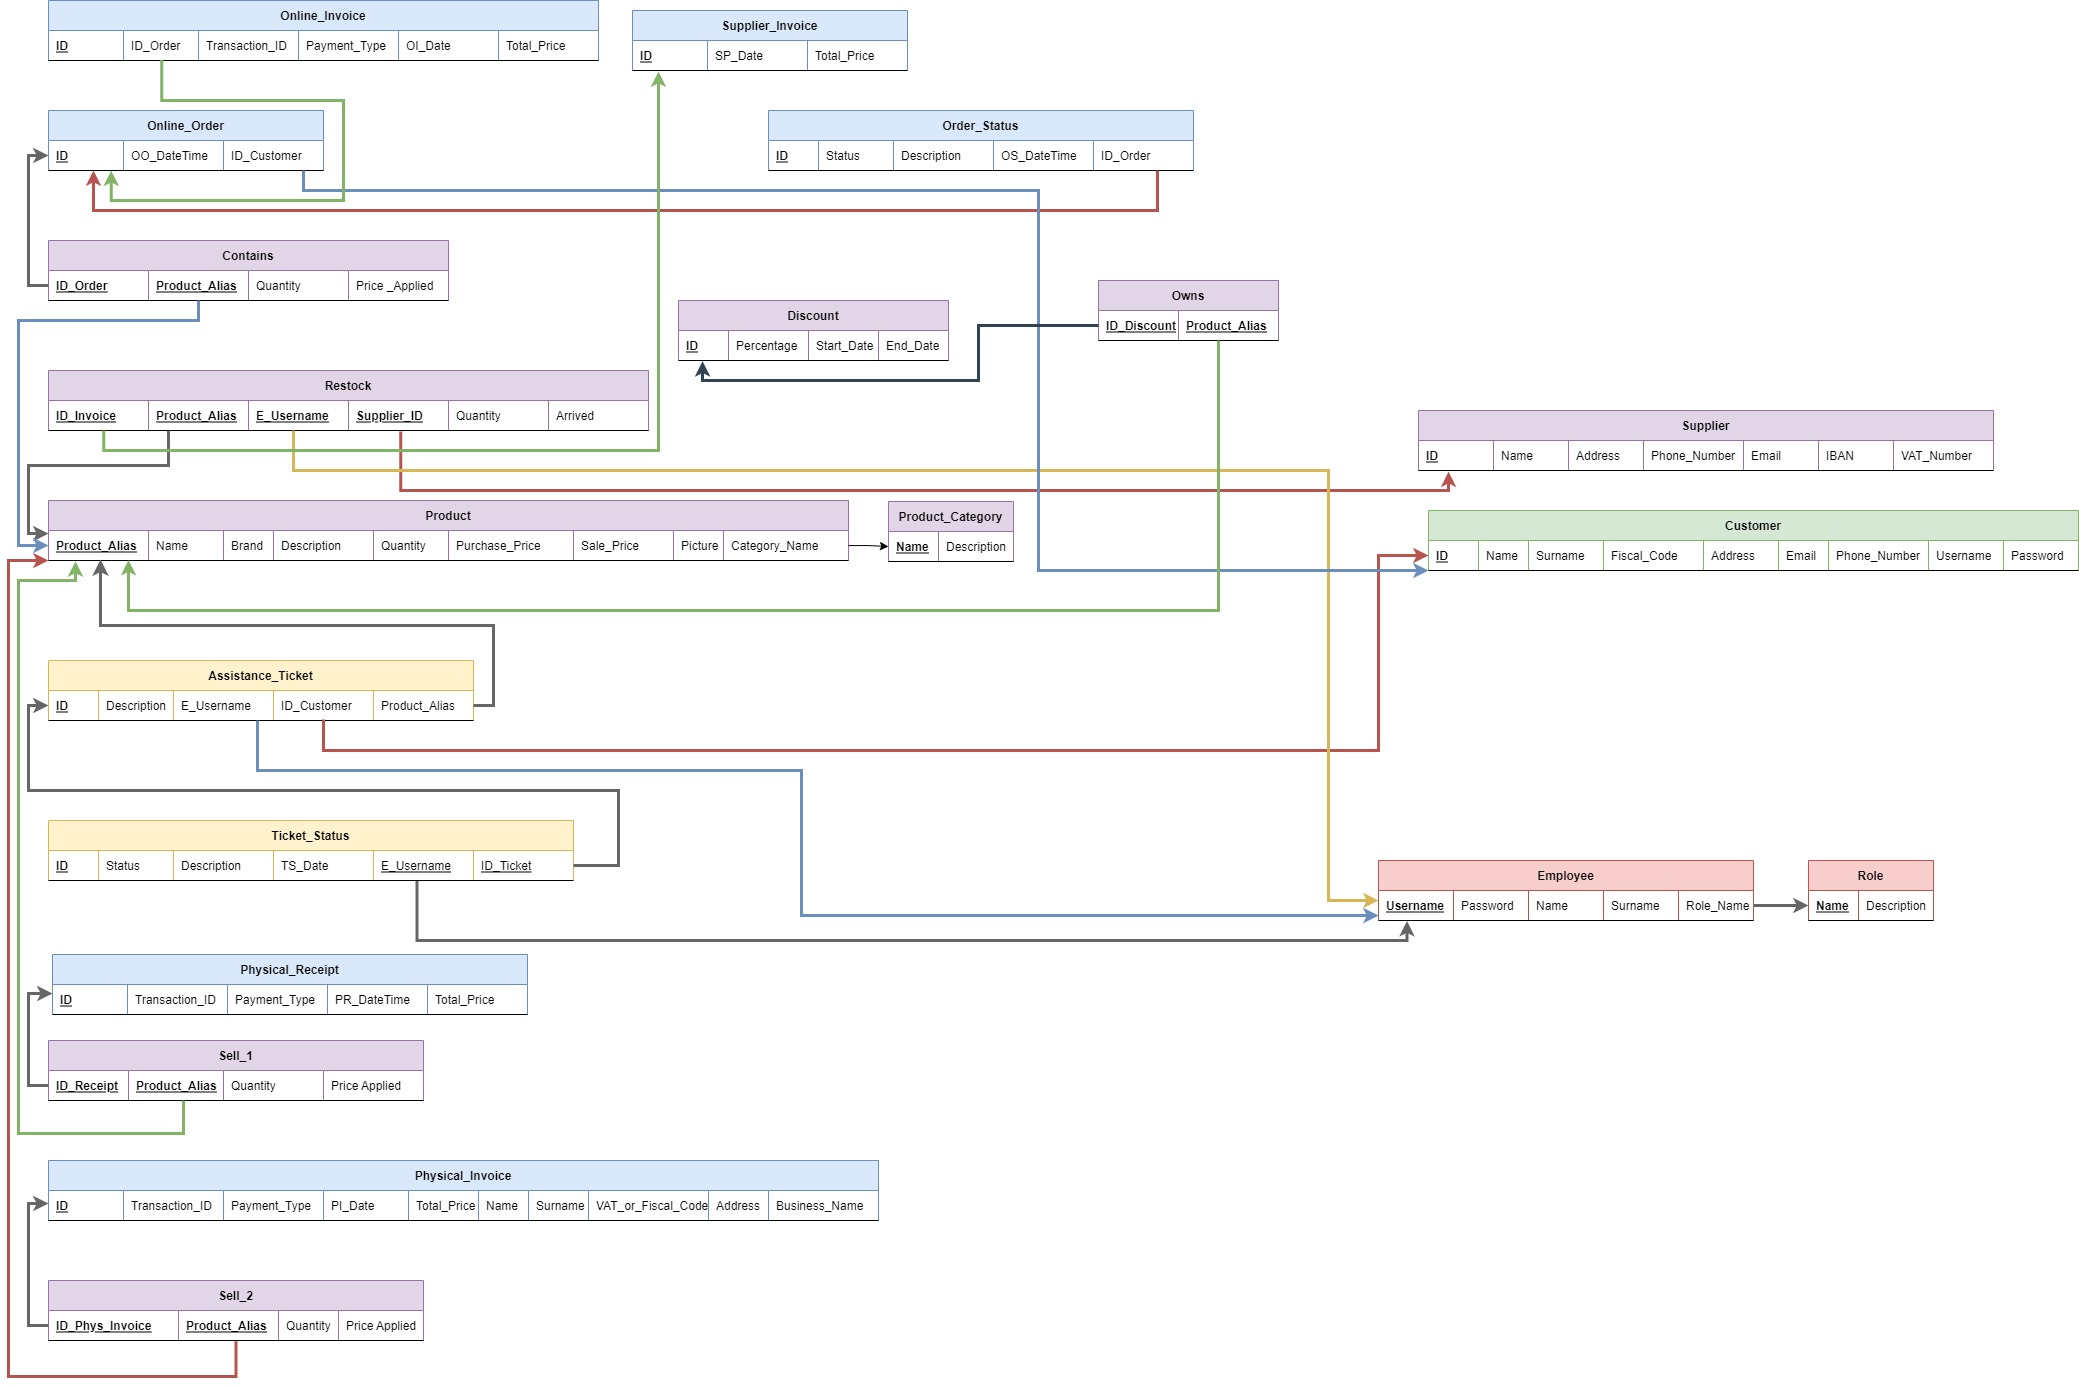
\includegraphics[width=17cm]{Schemas/LogicRS_original.jpg}
\caption{Relational schema designed by e-team}
\label{ls_original}
\end{figure}

In order to mantain the project manageable, we decided to remove some parts. In particular we decided to remove all the "offline services" and we decided to built our web application only to manage the online store.
Another part we removed is the management of the supplier, dedicating the development of our project only to the services seen by the client of the shop (excluding the management of the employes that is need in our webapp in order to setting up the permission.). In figure \ref{er_modified} and \ref{ls_modified} are reported the final version of the design for the data layer(ER schema and relational schema respectively).

\begin{figure}[H]
\centering
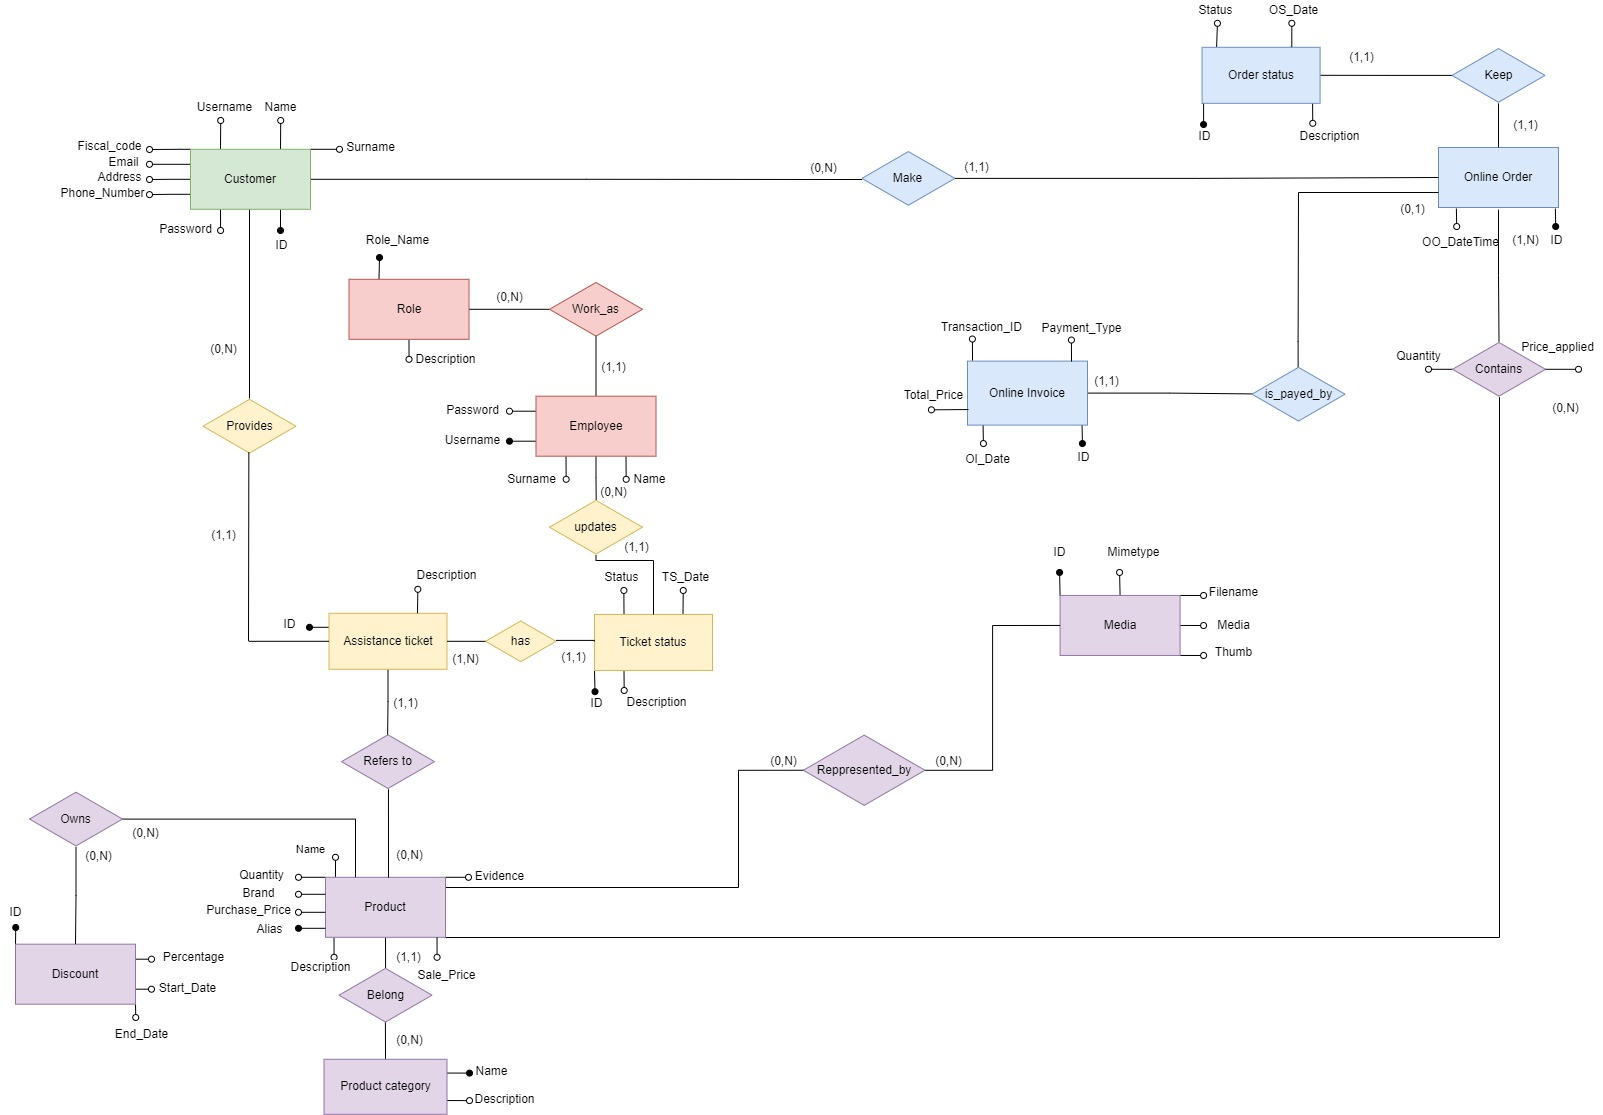
\includegraphics[width=17cm]{Schemas/ER_modified.jpg}
\caption{ER schema designed by e-team}
\label{er_modified}
\end{figure}

\begin{figure}[H]
\centering
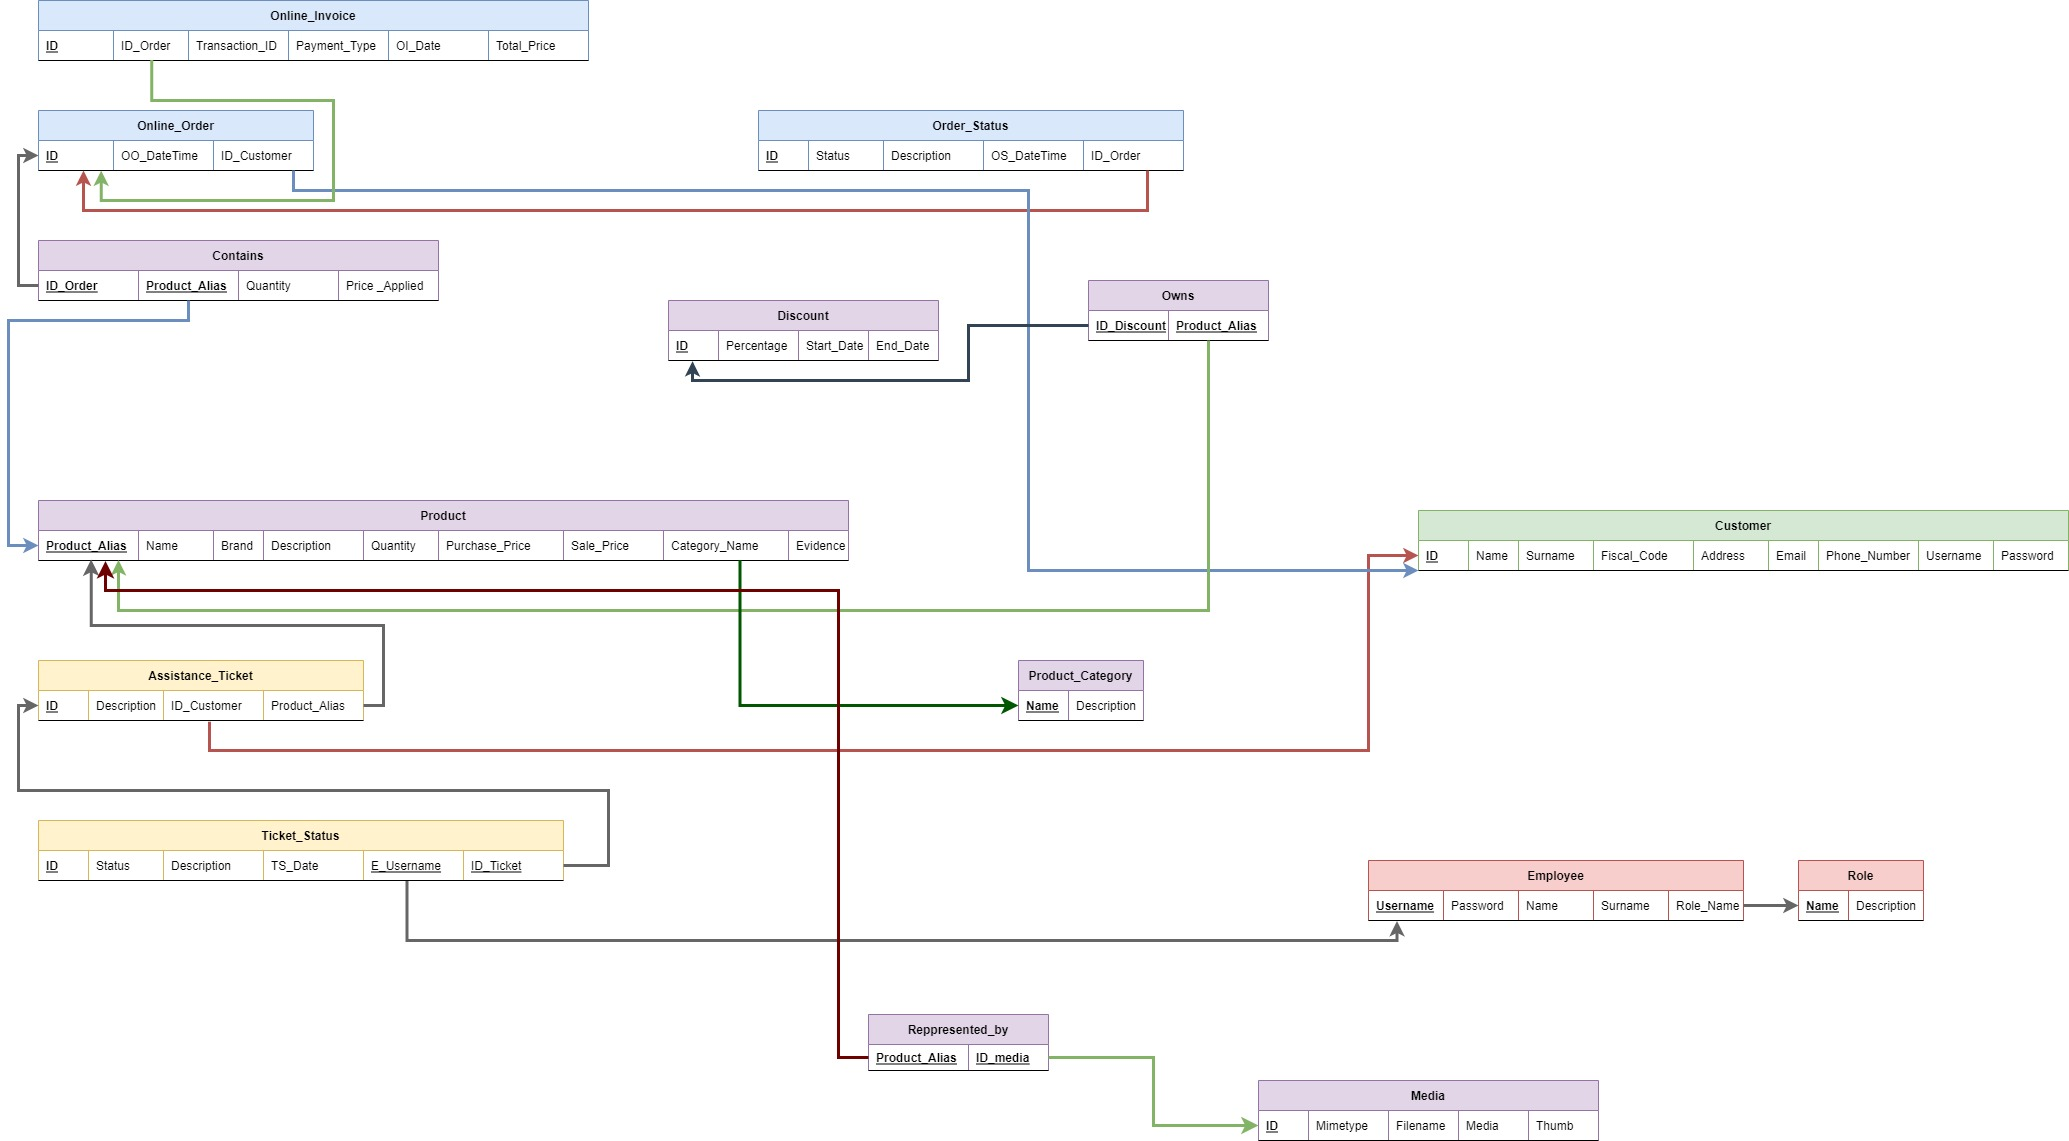
\includegraphics[width=17cm]{Schemas/LogicRS_modified.jpg}
\caption{Relational schema designed by e-team}
\label{ls_modified}
\end{figure}